\chapter{Final Design Overview}\label{chapter:finaldesign}
The overall exergame development was user centered. Based on the feedback gathered from the prototype game review (ref), discussions with experts (ref), and literature review (ref), new movements have been introduced and modifications have been made to the existing design in order to make the exergame engaging, enjoyable, and more intuitive to use and interact with. This section outlines the design and development of the final version of the Immotion exergame for warm up routine guidance and motivation.
\section{A Modular Design Approach}
In order to make the exergame easily adjustable and compliant with the user requirements, in our exergame design and development we followed a modular design approach. That is, each movement (exercise) that was required from the user to be performed is encapsulated in one distinct game segment. To put it differently, the whole game system was subdivided into smaller parts that could be independently created and then used accordingly. That way, by combining multiple segments randomly, we were able to generate a unique game map each time the user played the exergame. The end result of this approach was that our game is not constrained by one global map, but a dynamic one created on each game run. Moreover, having segments as the basic game blocks allowed us to easily add new segments that could make the game richer and the set of required movements bigger. Also, this way we could easily discard segments and movements users disliked or were difficult to perform. We believe this is a major feature that makes our exergame scalable and extensible for future user requirements and preferences. 
\section{Discussions With Fitness Experts}
During the development of our exergame, fitness and exercise experts were consulted in order to design game segments that would require movements often performed before physical activity and be effortlessly executed by the users without prior exercise knowledge. Based on their comments we also updated existing segments so the movements that is required to be executed is intuitive for the user and does not require further explanation. The modular design approach allowed us to easily add segments that required movements suggested by the experts at the spot and modify existing ones. Figure \ref{fig:expDesign} captures one of our discussions with a fitness expert.\\  
 \begin{figure}[h]
    \centering
    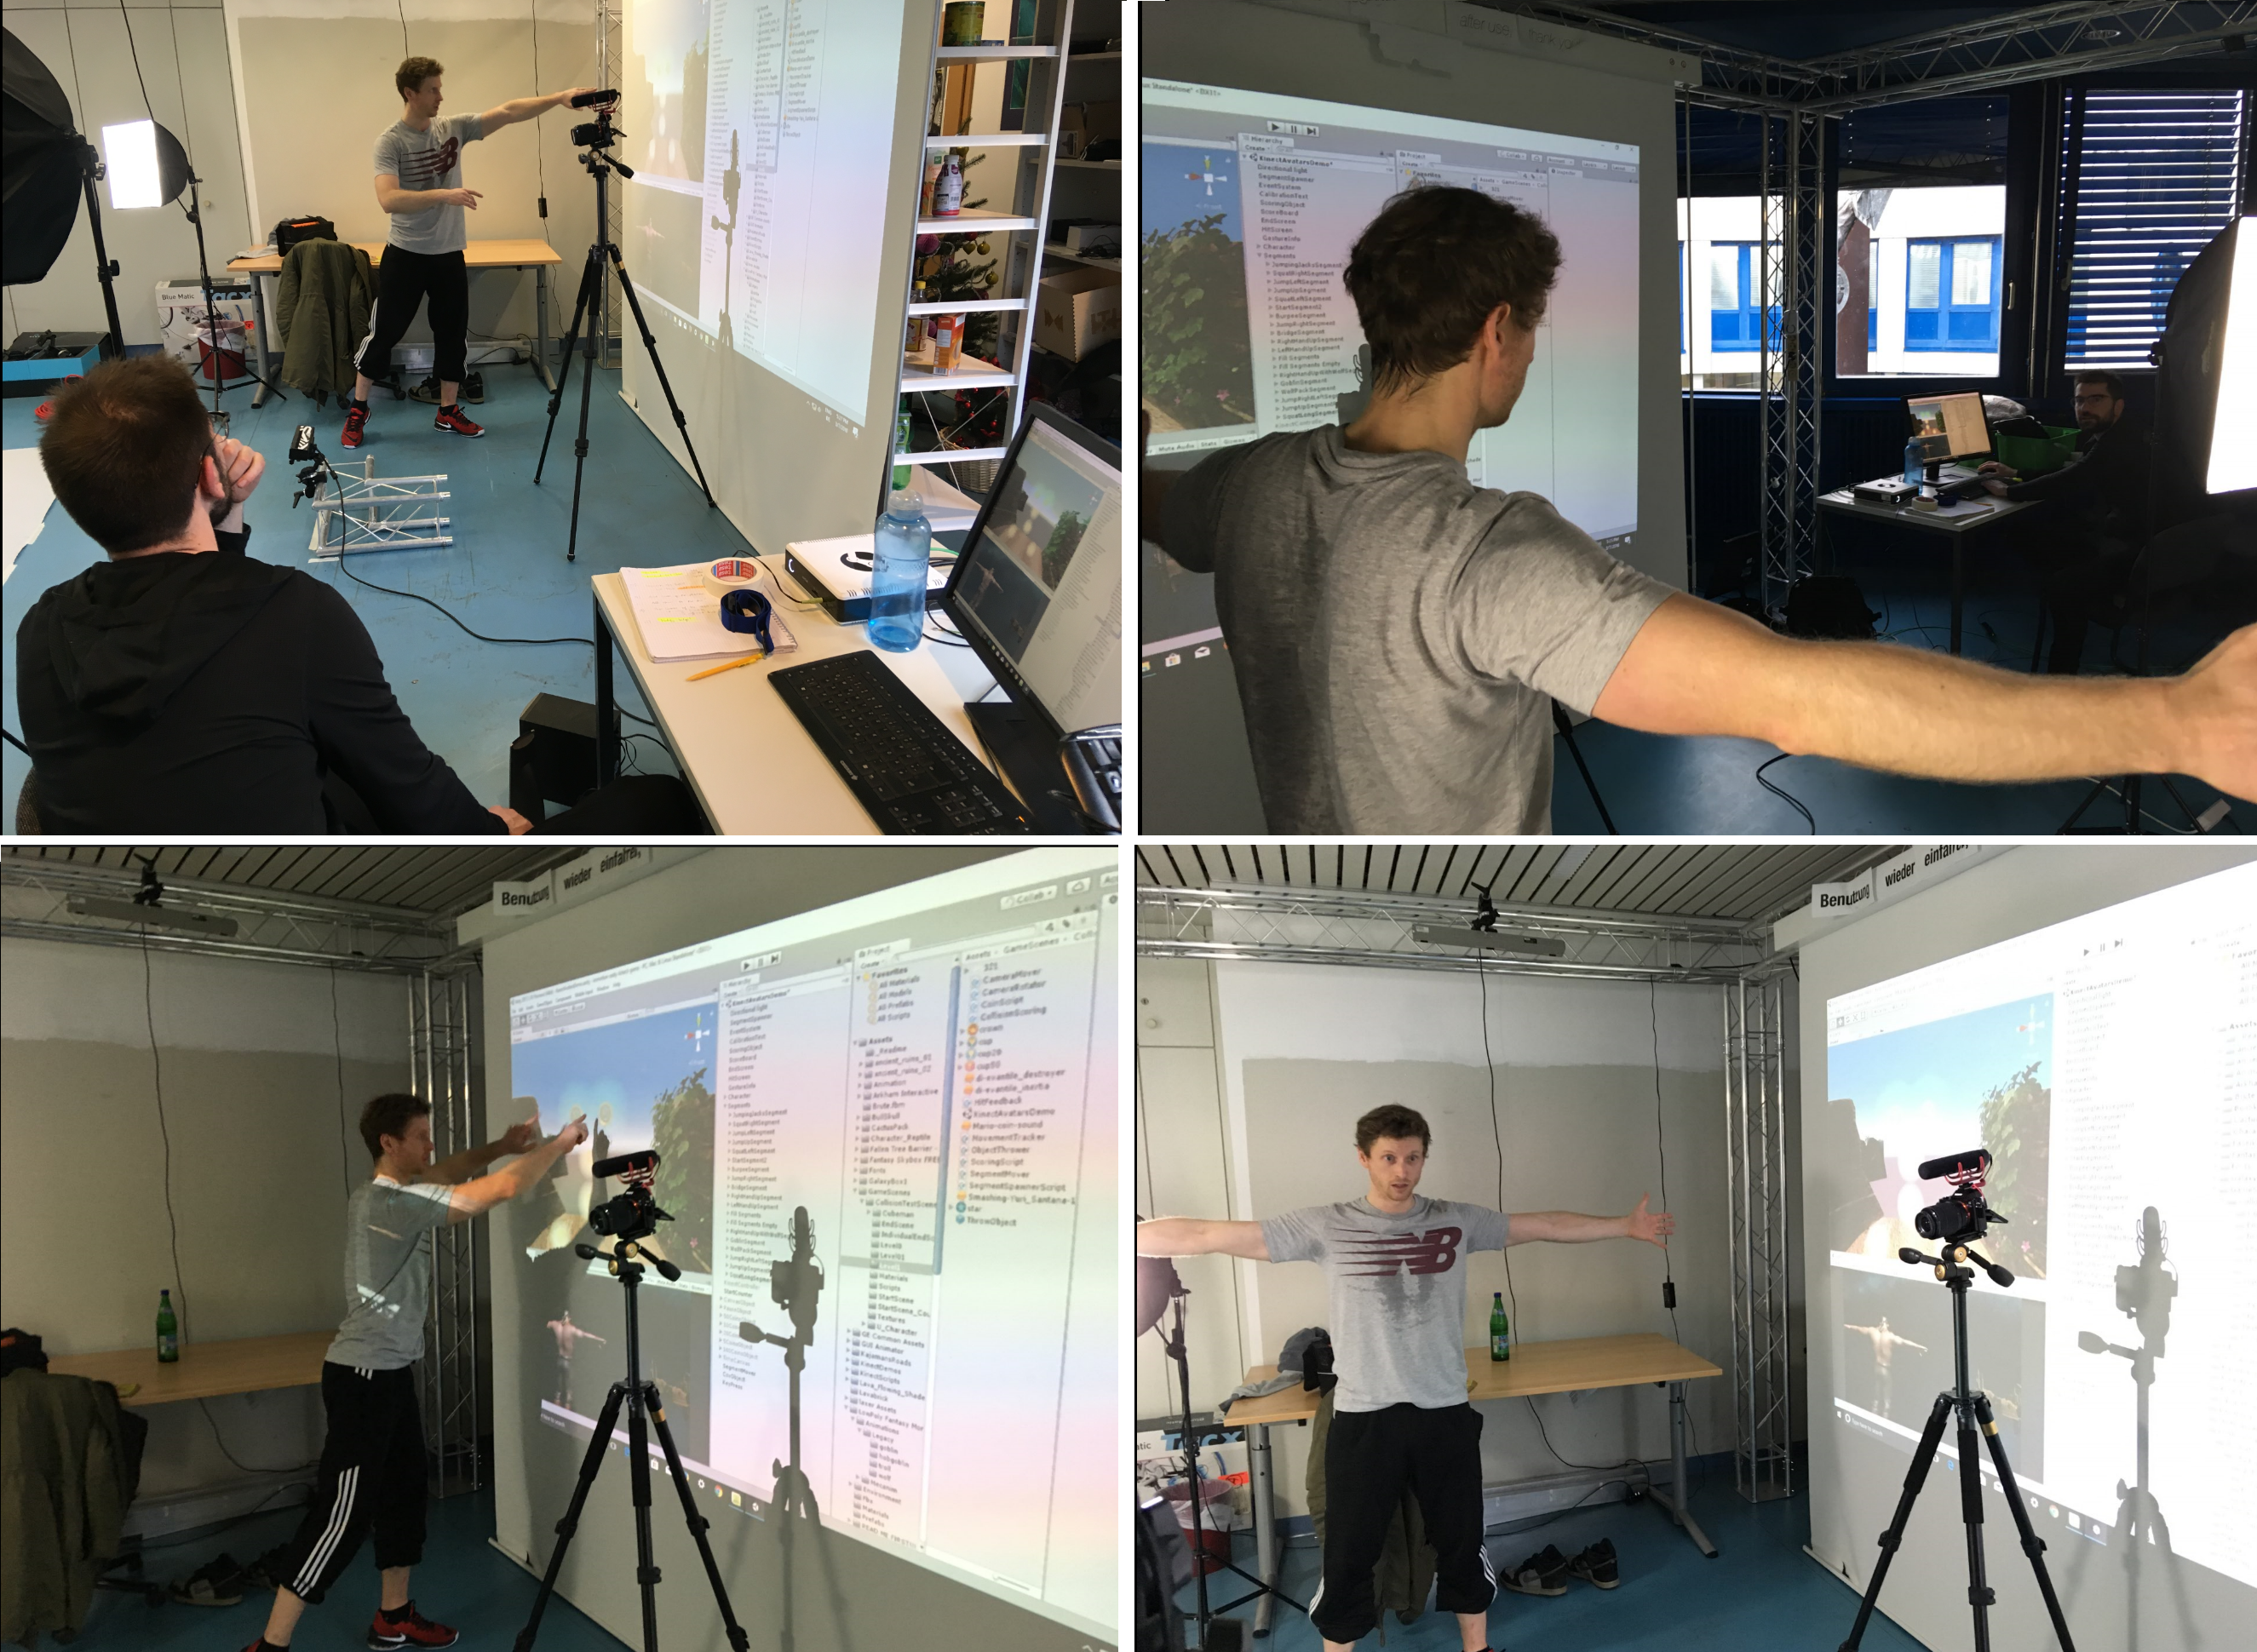
\includegraphics[width=\textwidth]{expertsDesign}
    \caption{Exergame related design discussions with fitness expert.}
    \label{fig:expDesign}
\end{figure}\\
In the next sections we describe and present the segments created as well as the movements that were required to be performed within them.\pagebreak
\section{Home Window Overview}
When the user starts the exergame, the \textit{Home screen} that is depicted in Figure \ref{fig:start} is showed. Apart from starting the game, other options are available for the user as well:
\begin{itemize}
\item Start
\item Help
\item Volume
\item High Score
\item Quit
\end{itemize}
\begin{figure}[h]
    \centering
    \includegraphics[width=\textwidth]{Start}
    \caption{Home screen.}
    \label{fig:start}
\end{figure}
Each of the above presented option opens a new window and provides the user with certain functions. Next, the above listed options will be further detailed.\pagebreak
\paragraph{Start Menu}
By selecting the \textit{Start} button in the Home screen, the user is presented with a new screen as showed in Figure \ref{fig:userinfo}. In this step, the user needs to input a username that will be used throughout the gameplay. The username does not have to be unique. In case it already exists, at the end of the game, all the scores achieved in previous game runs with the same username will be presented in ascending order by game scores as presented in Figure \ref{fig:individualScore}. By selecting \textit{Start} the exergame begins. By selecting \textit{Back}, the user is directed back to the Home screen.\\
\begin{figure}[h]
    \centering
    \includegraphics[width=\textwidth]{EnterName}
    \caption{User Info Menu.}
    \label{fig:userinfo}
\end{figure}
\paragraph{Help Menu}
The Help menu, as presented in Figure \ref{fig:help} lets the user know how to interact with the game, change the speed of the game, and start or stop the game. It also contains contact information for error reporting and user feedback. The Back button allows the user to go back to the Home screen.
\begin{figure}[h]
    \centering
    \includegraphics[width=\textwidth]{Help}
    \caption{Help menu.}
    \label{fig:help}
\end{figure}
\paragraph{Volume Menu}
The volume menu showed in Figure \ref{fig:volume}, gives users the possibility to modify the volume of the exergame's background music and sound effects (coins and obstacle collision sounds).\\
\begin{figure}[h]
    \centering
    \includegraphics[width=\textwidth]{Volume}
    \caption{Adjust volume menu.}
    \label{fig:volume}
\end{figure}
\paragraph{High Score Menu}
The high score menu depicted in Figure \ref{fig:highscore} ranks the users who played the exergame based on the points collected during one gameplay. The leaderboard displays the user's rank, name, score, and duration. This is a global leaderboard and it is different than the one presented in Figure \ref{fig:individualScore} since it includes all the users previously interacted with the game, their scores, and duration they played the game. Contrarily, the individual score board, displayed only at the end of each gameplay, shows the score and game duration of the user who currently interacted with the exergame. The Back button allows the user to go back to the Home screen.
\begin{figure}[h]
    \centering
    \includegraphics[width=\textwidth]{HighScore}
    \caption{High score menu.}
    \label{fig:highscore}
\end{figure}
\paragraph{Quit Menu}
The quit menu button was used for ending (closing) the game. 
\section{Game Start Overview}
For the purpose of tracking progress and achievements over time, users are required to input a name or username they would like to use during the gameplay. Based on the username, we display user's current score and position on the leaderboard during the gameplay and the highest scores at the end of the gameplay. The live score board and the leaderboard are presented  in Figure \textit{Individual score board} and Figure \ref{fig:individualScore}. After the user set the username and pressed the Start button, a \textit{Countdown window} as showed in Figure \ref{fig:counter} is presented to the user. The duration of the countdown is set to 5 seconds. We opted for this duration because it showed as the most optimal in our pilot study previously conducted with the university personal. This amount of time was sufficient for the users to prepare for the upcoming exercise by moving to the correct position. In case the user was not in the Kinect sensor range at the beginning of the game, a popup information window was displayed as showed in \ref{fig:waiting}. This information window was also displayed in case the connection to the Kinect sensor failed during the gameplay. \\
\begin{figure}[h]
    \centering
    \includegraphics[width=\textwidth]{Counter}
    \caption{Countdown window.}
    \label{fig:counter}
\end{figure}\\
\begin{figure}[h]
    \centering
    \includegraphics[width=0.6\textwidth]{LiveScore}
    \caption{``Live score'' during gameplay displayed in the left corner.}
    \label{fig:livescore}
\end{figure}\\
\begin{figure}[h]
    \centering
    \includegraphics[width=\textwidth]{WaitingForUser}
    \caption{``Waiting for user'' popup window.}
    \label{fig:waiting}
\end{figure}\\
Next, an overview of the game segments and corresponding movements required to perform in each of them will be presented.
\section{Game Segments Overview}
As already pointed out, each warm up movement the user was required to perform has been represented by a game segment. Following recommendations from experts, available literature, and the previously conducted online study, the list of warm up movements the users were required to perform during the game was updated. Additionally, we introduced so called \textit{filler} or \textit{empty} segments. In these segments no movements were required to be performed. They were placed between regular segments where movements needed to be performed. Their only purpose was to give users a short amount of time to prepare for the subsequent game segment. By generating all the segments randomly during gameplay, each resulting game map and warm up session induced by the map were unique. Moreover, our intention was to make the exergame intuitive to use. That is, the movements should come naturally to the users and should not require additional explanation. This was the result of our iterative and user centered design approach. We designed the segments based on the movements that can help users to warm up, and not contrarily. That way, every movement induced by obstacles and coins was executed correctly and came naturally to the player without additional explanation. Figure \ref{fig:topview} gives an overview of all the segments used in the exergame.\pagebreak
\begin{figure}[h]
    \centering
    \includegraphics[width=\textwidth]{SegmentsTopView}
    \caption{Overview of game segments - top view.}
    \label{fig:topview}
\end{figure}\\
In most of the segments depicted in Figure \ref{fig:topview}, one specific movement was required to be performed. Some segments were without obstacles and were present in order for the users to prepare for the next segment (and movements). Also, segments without any obstacles were used at the beginning of the exergame. At the very beginning of the exergame, ten filler segments were generated, however this number has been made adjustable. The empty segments were placed at the beginning in order to avoid any sudden movements by the player risking injuries. Moreover, not having to perform any movements gave the player time to adjust to the gameplay and prepare for the movements.\\
All the segments were designed to induce one of the following movement:
\begin{itemize}
\item Left hand up
\item Right hand up
\item Squat (short and long)
\item Jump
\item Star jump
\item Left hand down to the floor
\item Right hand down to the floor
\end{itemize}
Figure \ref{fig:rightup} shows the segment in which the user is required to move the right hand in the upper position and, in the same time, avoid the obstacle. In case the user comes in contact with the obstacle, one point is substracted from the overall user's score.\\
\begin{figure}[h]
    \centering
    \includegraphics[width=0.85\textwidth]{RightHandUp}
    \caption{Right hand up segment.}
    \label{fig:rightup}
\end{figure}
\begin{figure}[h]
    \centering
    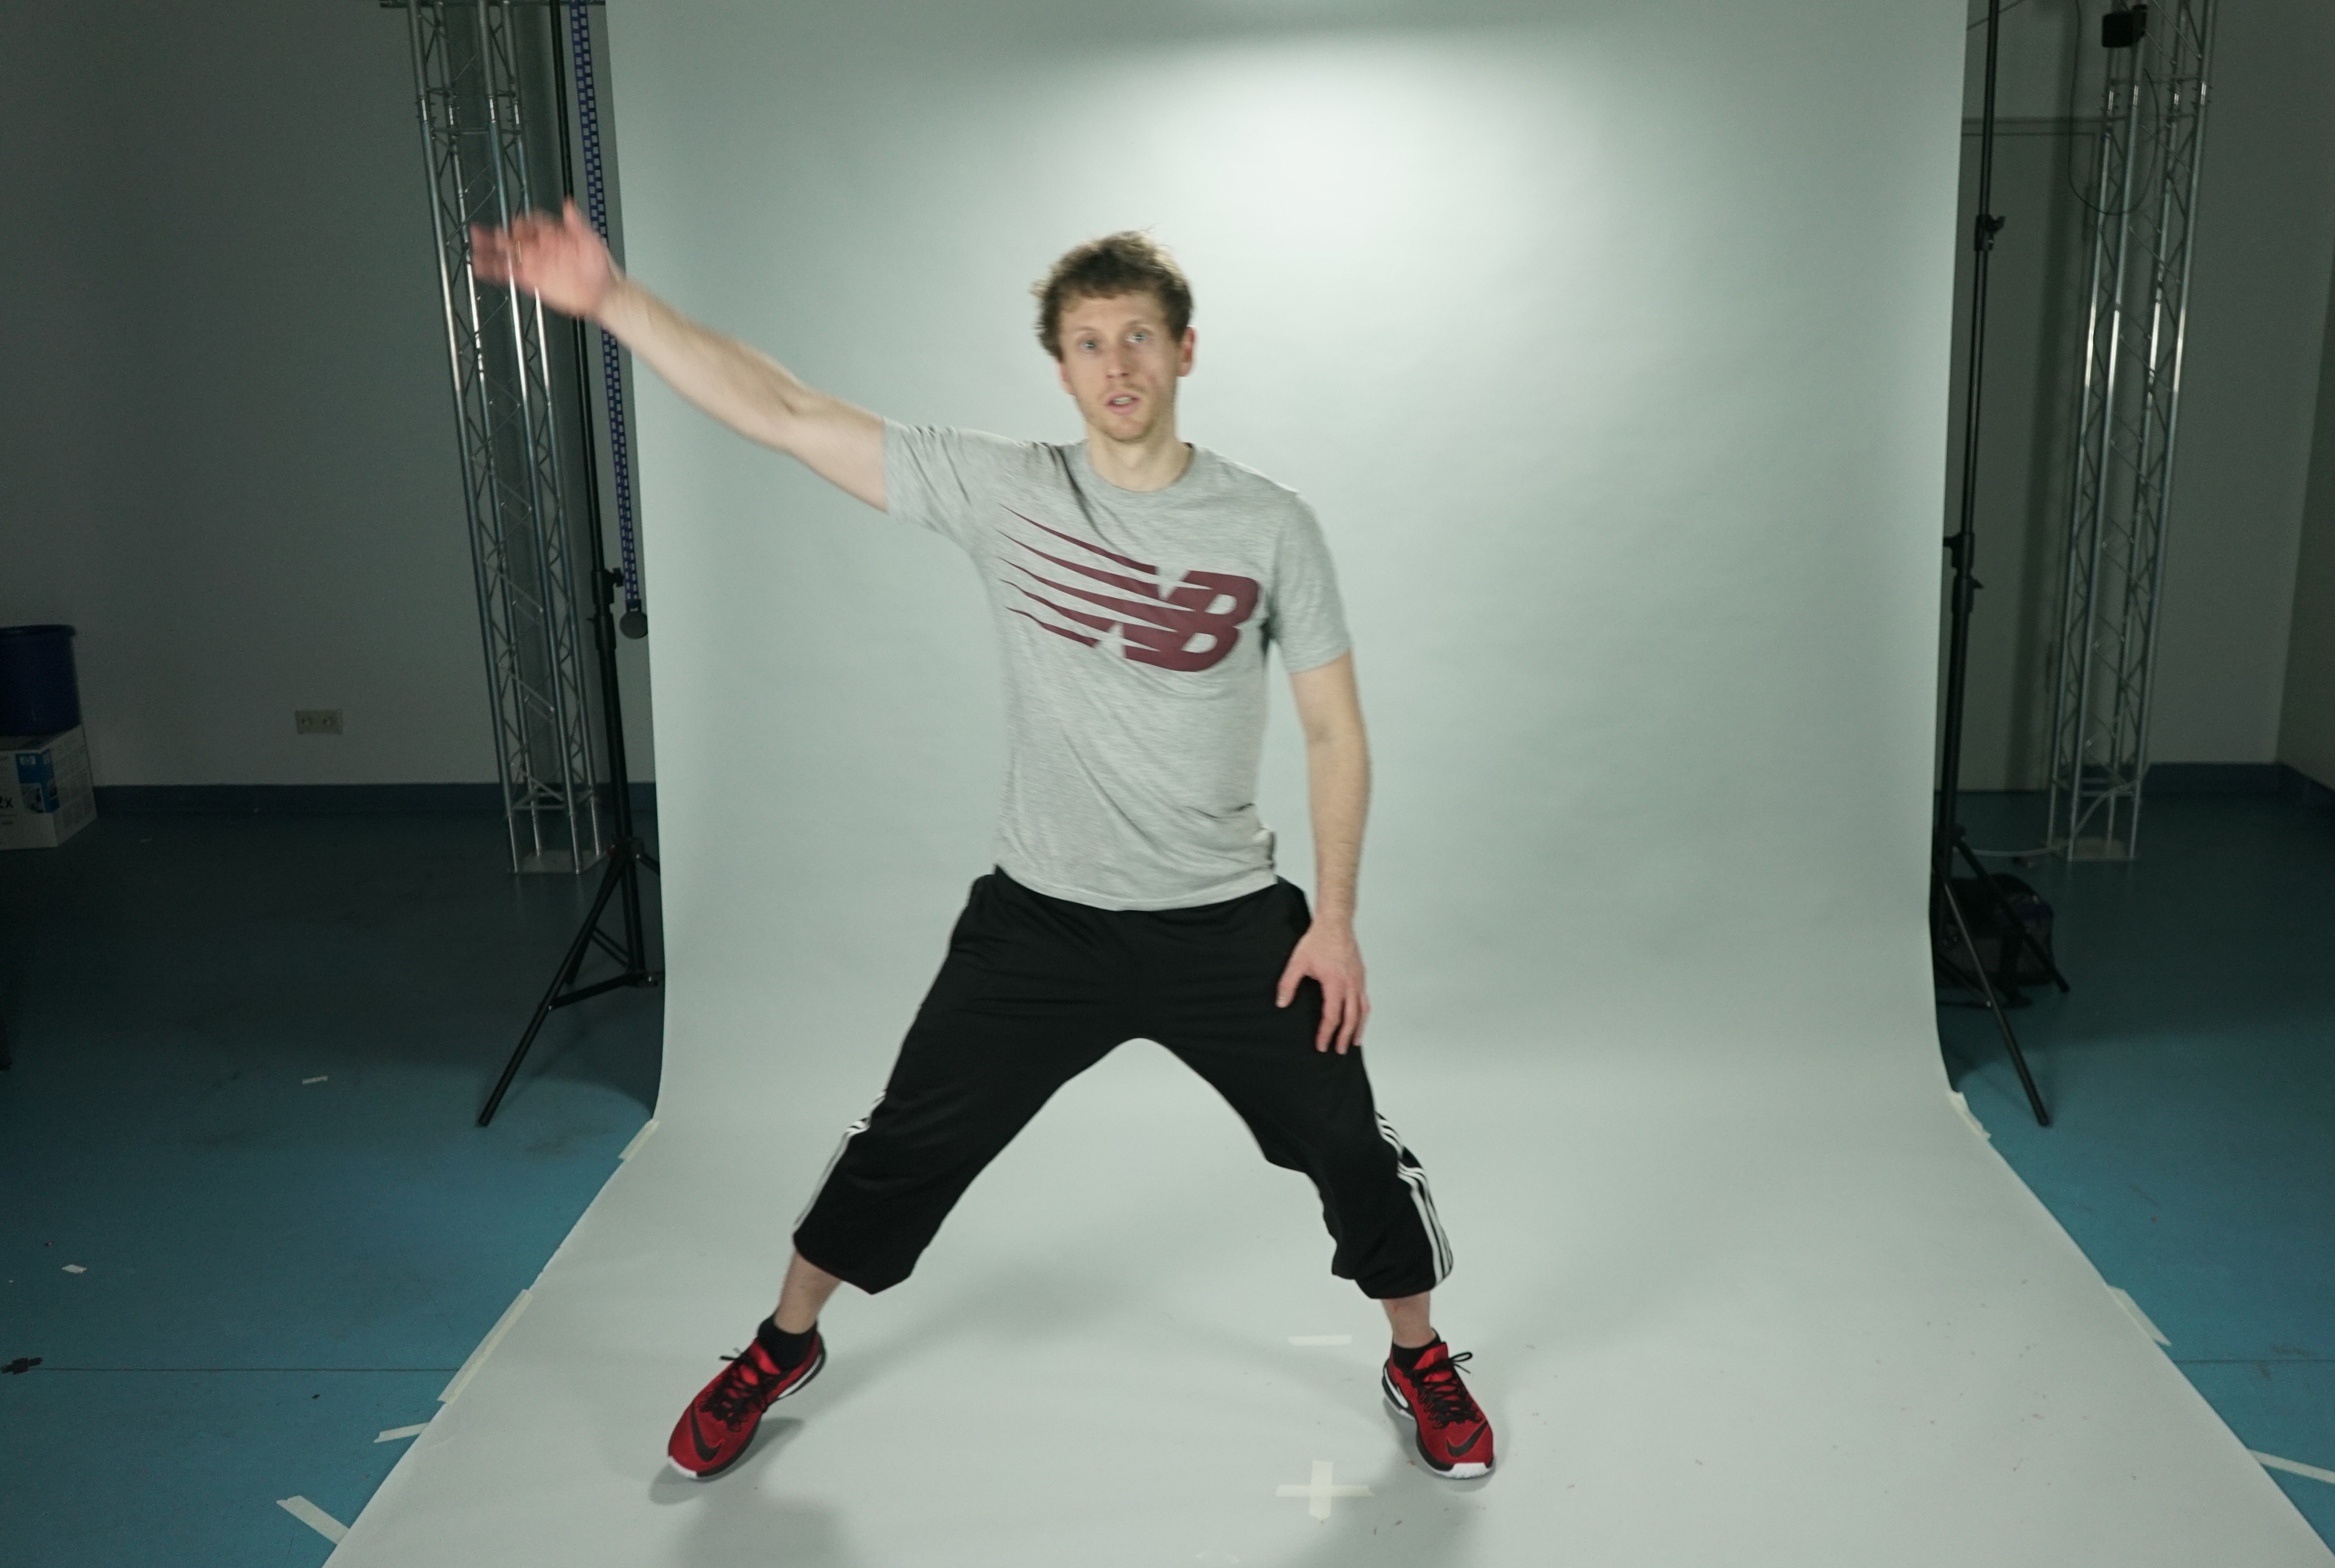
\includegraphics[width=0.85\textwidth]{ExpertRightHandUp}
    \caption{Expert right hand up movement.}
    \label{fig:rightHandUp}
\end{figure}\\\\
Figure \ref{fig:leftup} depict the segment in which the user is required to move the left hand in the upper position in order to collect the coins. The obstacle was placed below the coins and one point is reduced from the user's overall score in case it was hit.\\
\begin{figure}[h]
    \centering
    \includegraphics[width=0.85\textwidth]{LeftHandUp}
    \caption{Left hand up segment.}
    \label{fig:leftup}
\end{figure}
\begin{figure}[h]
    \centering
    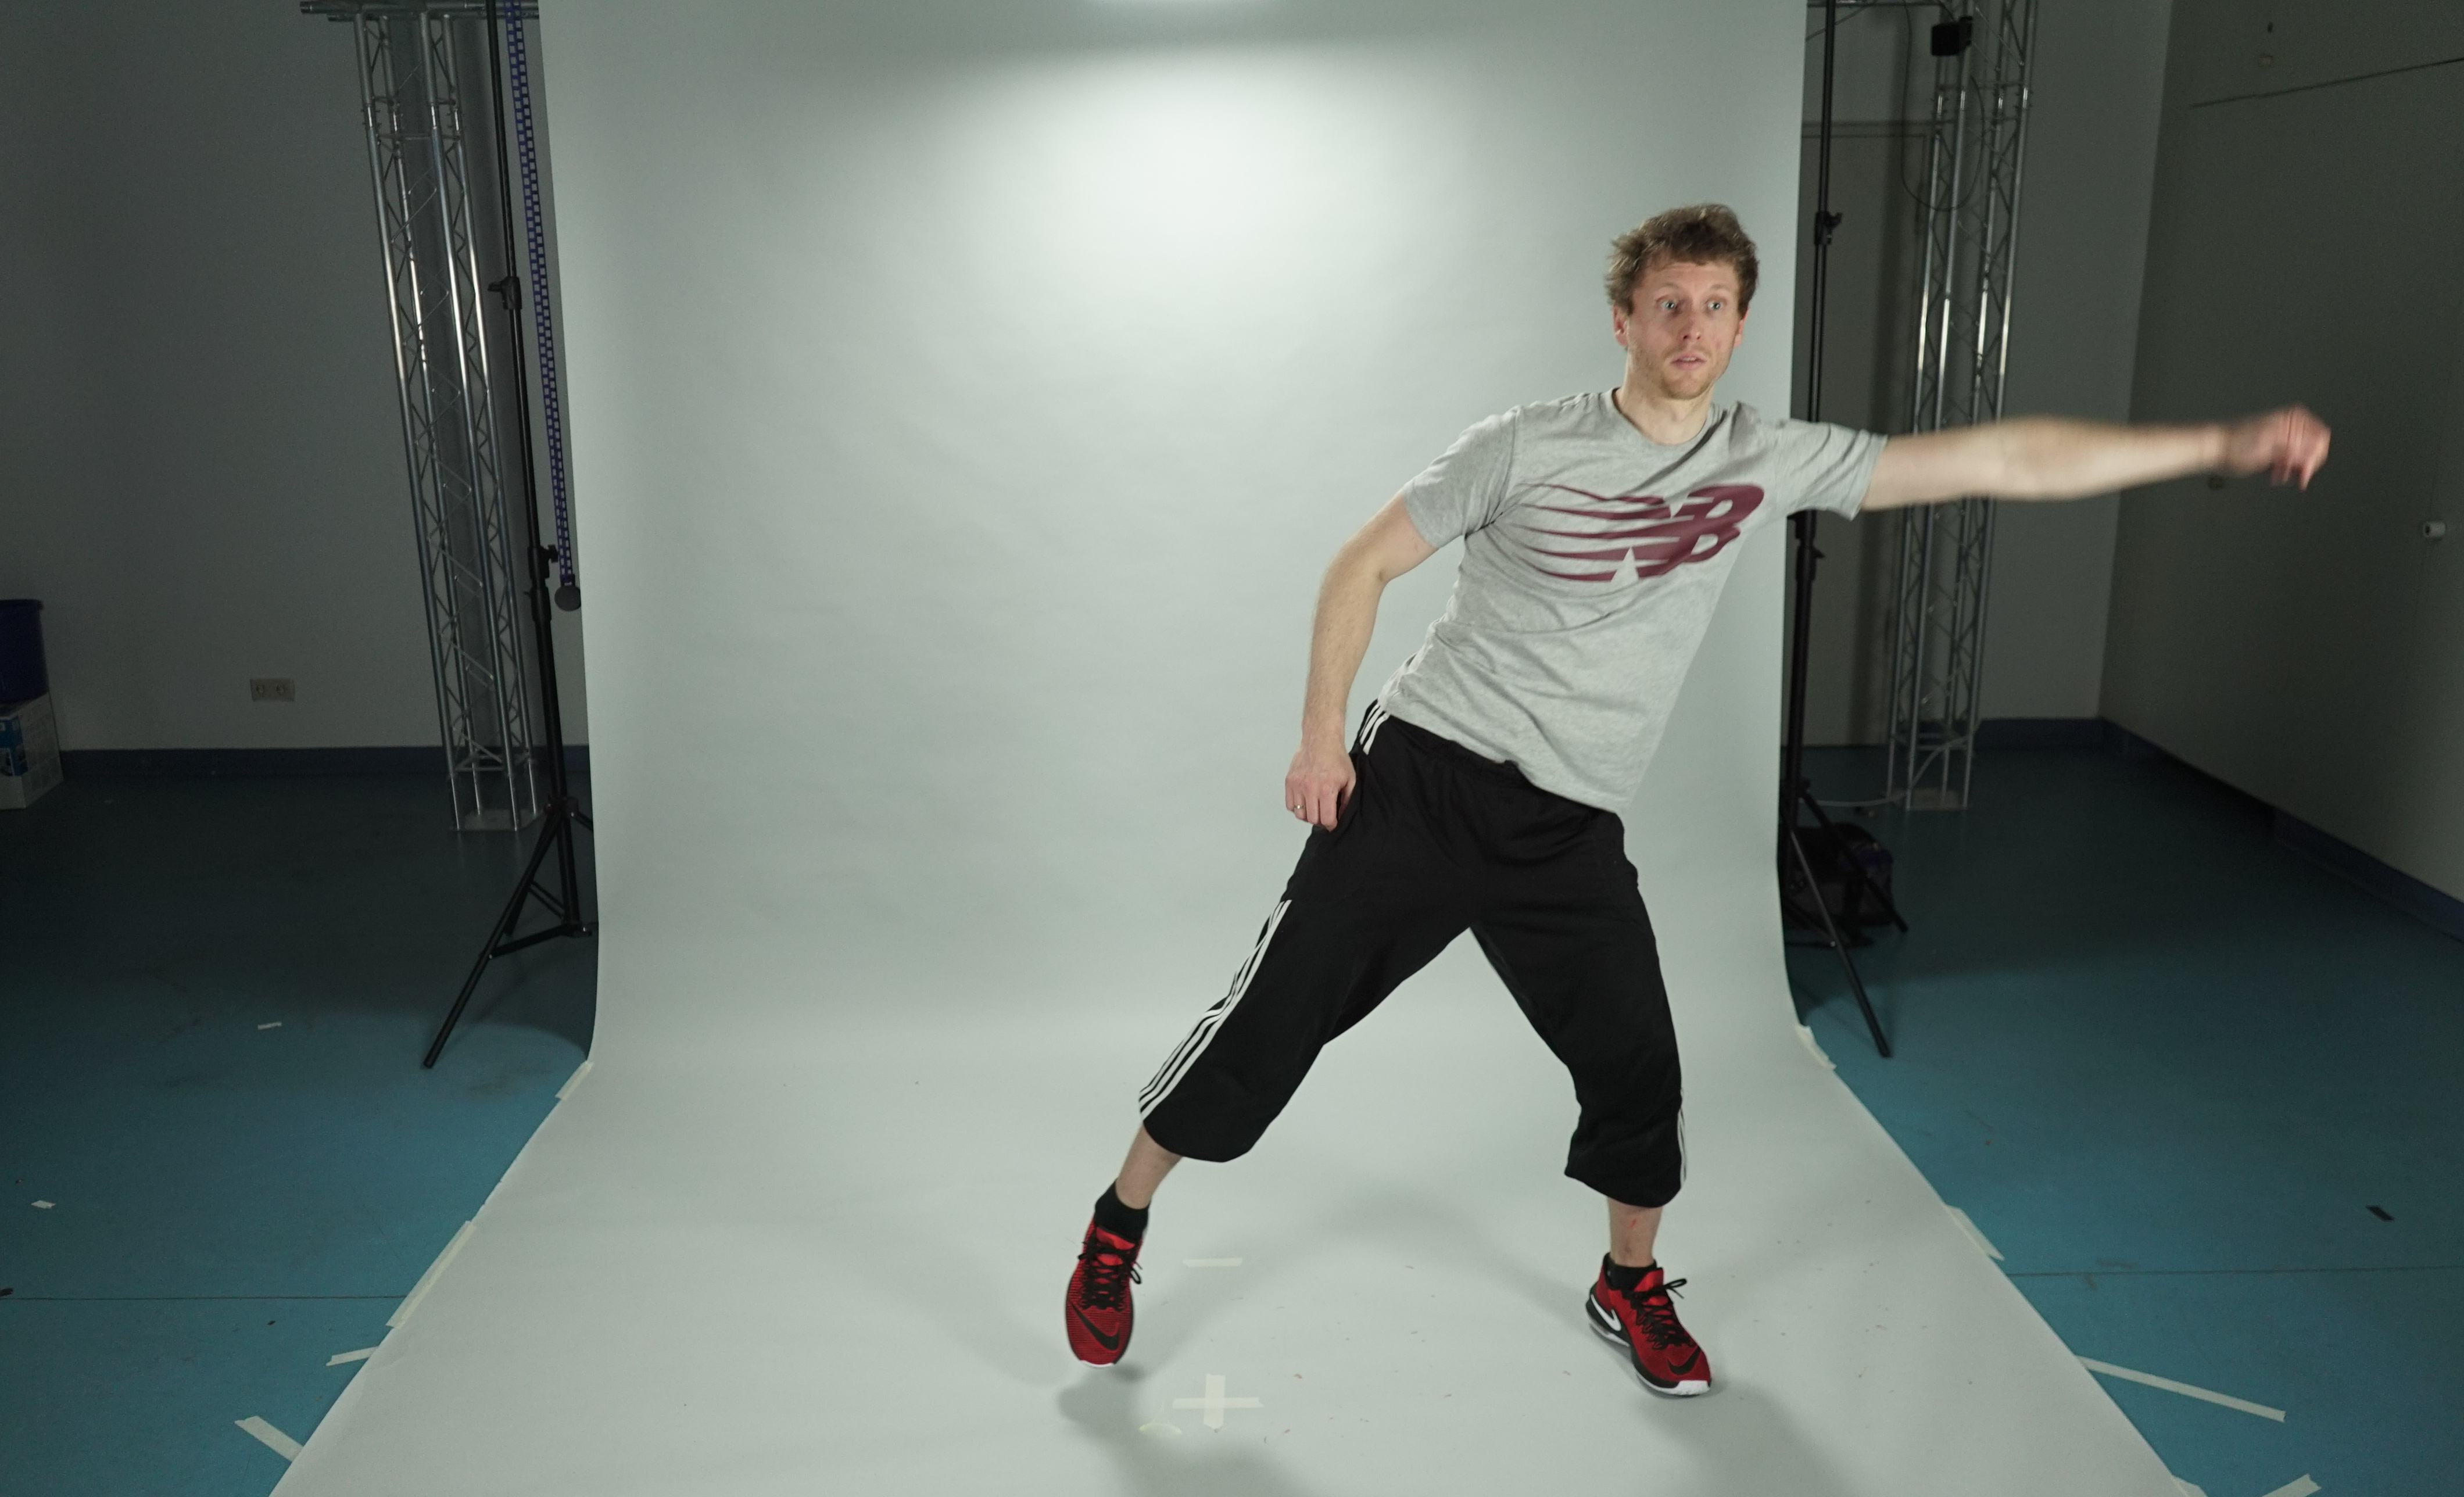
\includegraphics[width=0.85\textwidth]{ExpertLeftHandUp}
    \caption{Expert left hand up movement.}
    \label{fig:leftHandUp}
\end{figure}\\
In segments presented in Figure \ref{fig:wolfRight},  \ref{fig:goblin}, and \ref{fig:goblin} similar hand movements were required to be performed. The only difference was that in these segments the user is given a choice whether to go left or right. For instance, in Figure \ref{fig:goblin} player could collect four coins by moving to the right side. On the other hand, the user player could also go left and try to collect a blue coin that was worth five points. However, there was a possibility to lose points if collided with the obstacle.\\
\begin{figure}[h]
    \centering
    \includegraphics[width=0.85\textwidth]{HandUpRightWolf}
    \caption{Right hand up segment.}
    \label{fig:wolfRight}
\end{figure}
\begin{figure}[h]
    \centering
    \includegraphics[width=0.85\textwidth]{GoblinHandLeftOrRight}
    \caption{Right or Left hand up segment.}
    \label{fig:goblin}
\end{figure}\\\\
Figures \ref{fig:2wolfs} and \ref{fig:2sides} represent a segment where the player was also given an option to chose which movement to perform. Both the movements included rising hand in the upper position. The decision was left to the user. In case the user opted for the left side, the possible reward were two blue coins that were worth ten points in total. In case the user opted for the right side, the possible reward were three red coins that were worth nine points in total. However, there was a possibility to lose points by colliding with the obstacle.\\
\begin{figure}[h]
    \centering
    \includegraphics[width=0.85\textwidth]{2WolfsRight}
    \caption{Right or Left hand up segment.}
    \label{fig:2wolfs}
\end{figure}\\
\begin{figure}[h]
    \centering
    \includegraphics[width=0.85\textwidth]{TwoSides}
    \caption{Right or Left hand up segment.}
    \label{fig:2sides}
\end{figure}\\\\
In Figure \ref{fig:jumpleft} the user was required move to the left and touch the floor with the left hand in order to collect the coins. Moreover, the player was required to stay in that position for a short amount of time in order to collect all the coins.\\
\begin{figure}[h]
    \centering
    \includegraphics[width=0.85\textwidth]{JumpRight}
    \caption{Move left segment.}
    \label{fig:jumpleft}
\end{figure}
\begin{figure}[h]
    \centering
    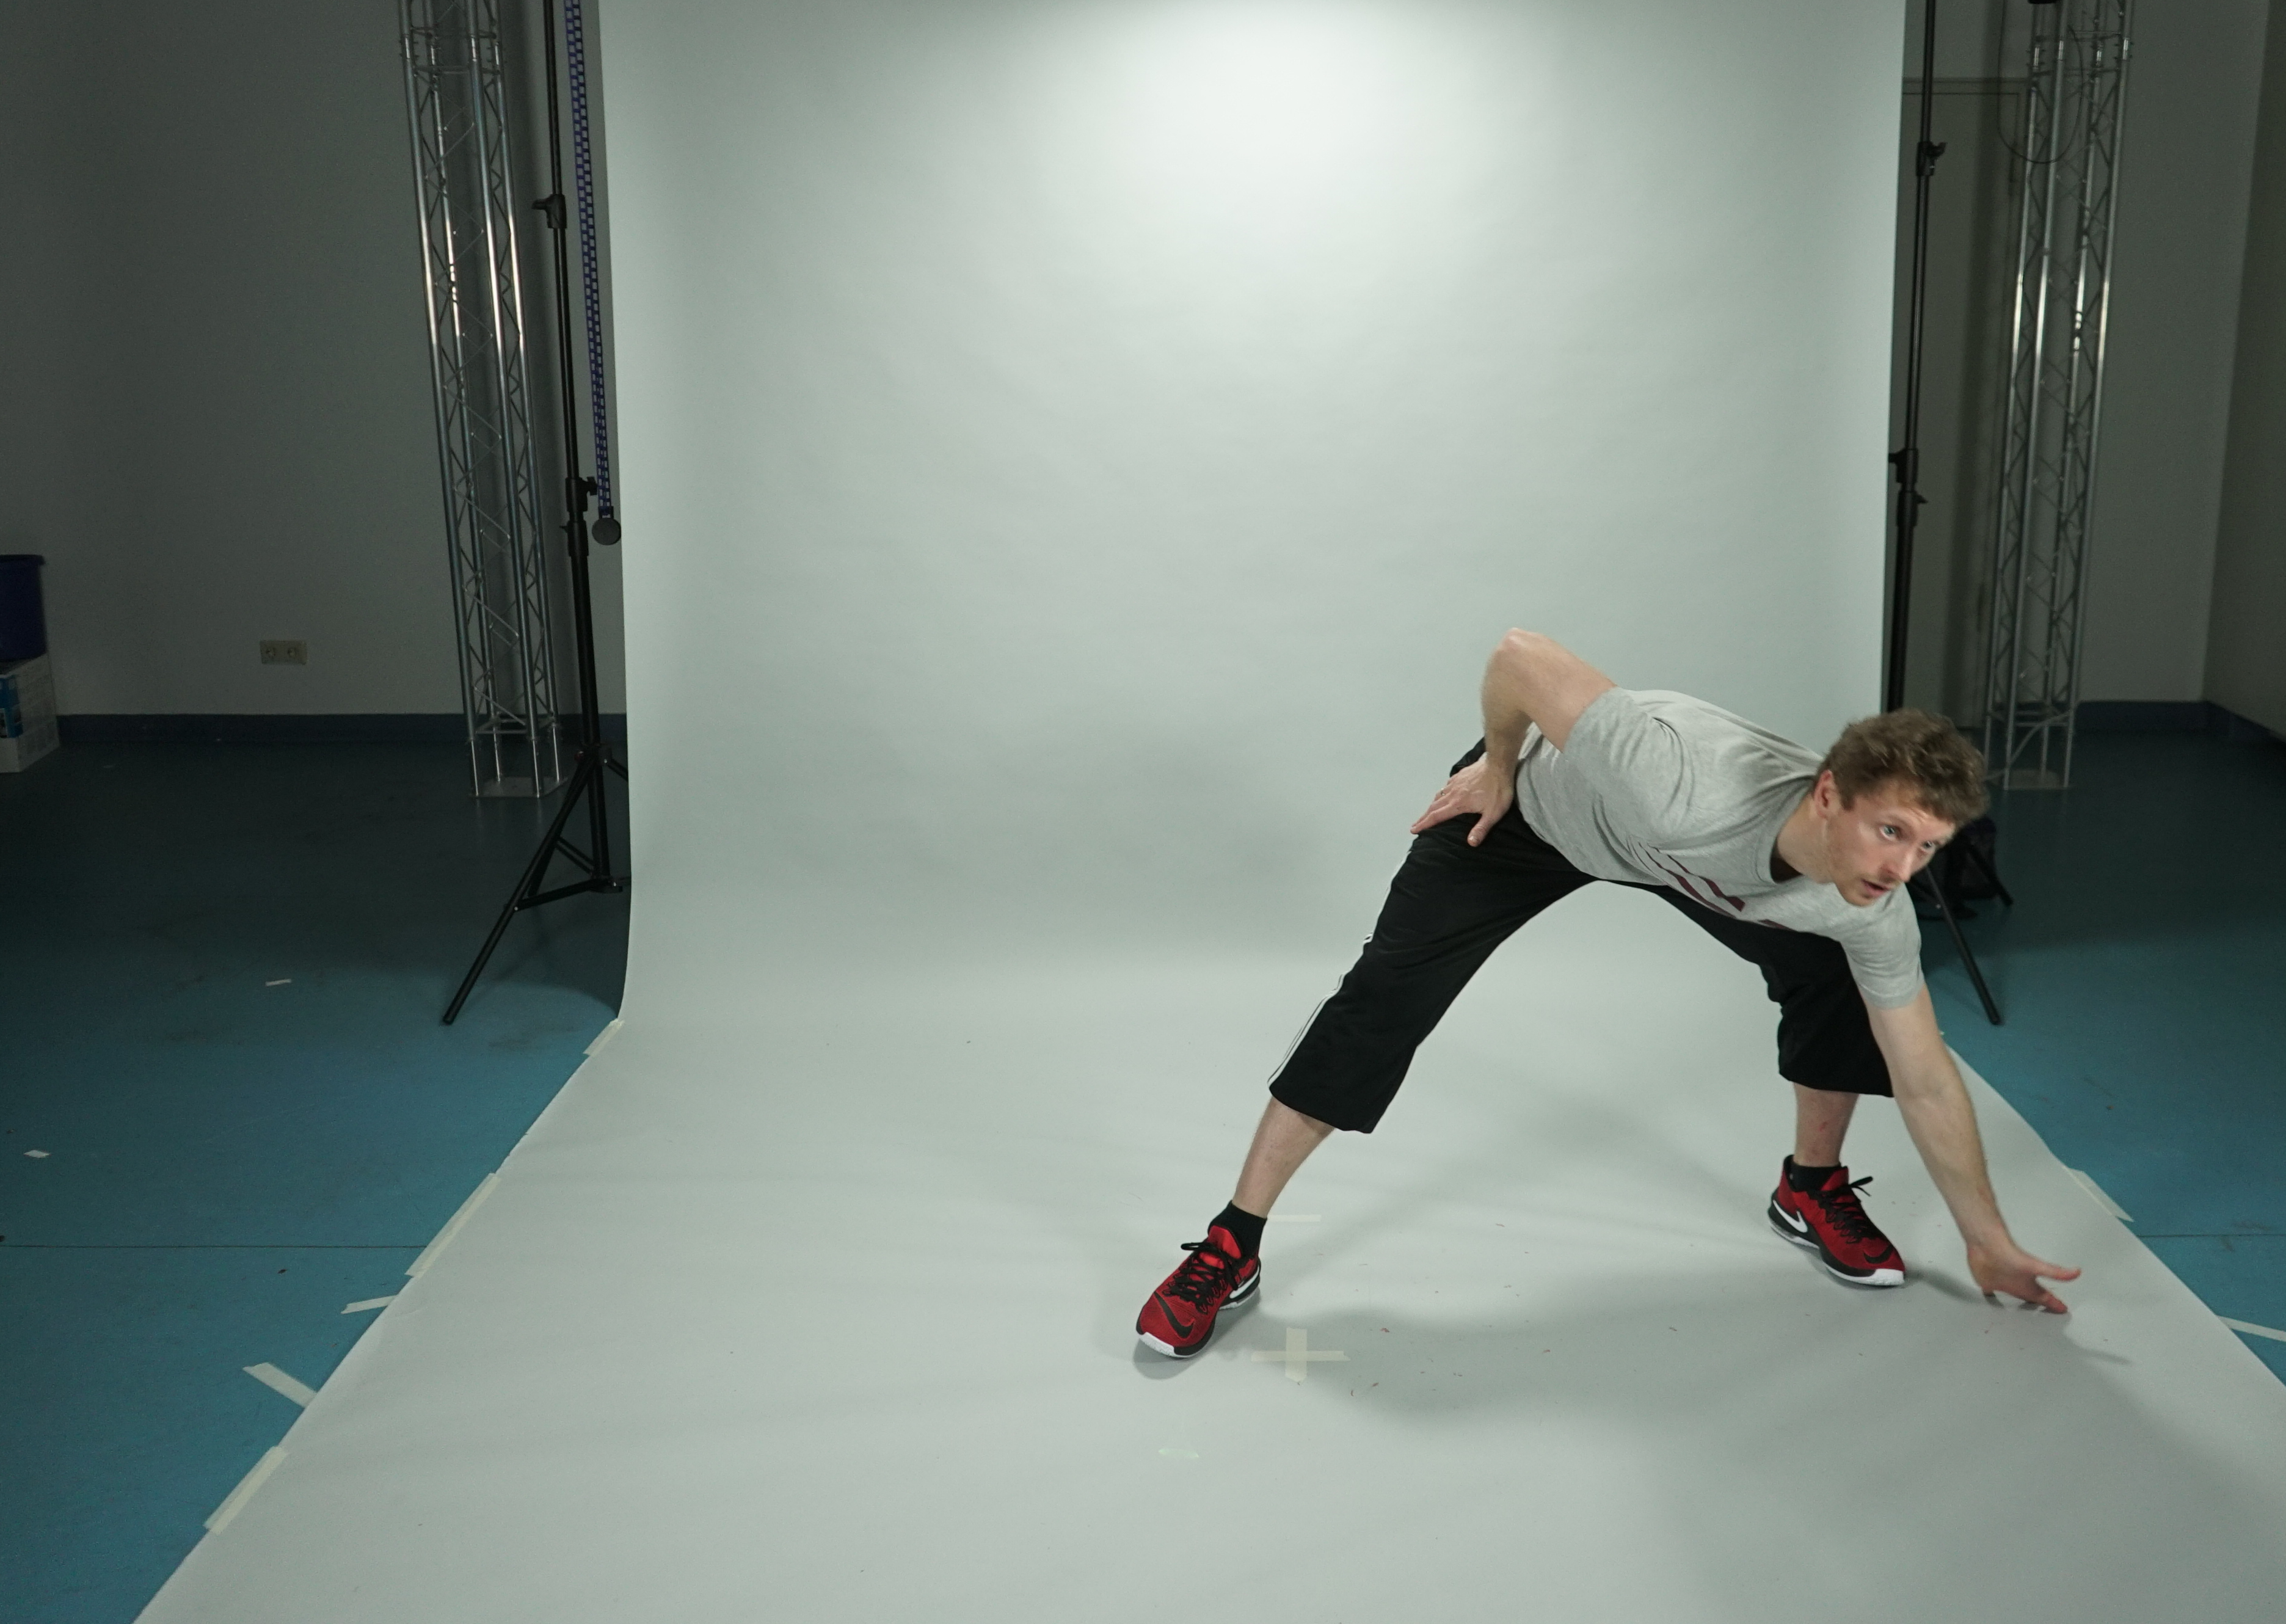
\includegraphics[width=0.85\textwidth]{ExpertHandDownLeft}
    \caption{Expert left hand down movement.}
    \label{fig:expertLeftDown}
\end{figure}\\
In Figure \ref{fig:jumpright} the user was required move to the right and touch the floor with the right hand in order to collect the coins. As in previous segments, in case an obstacle was hit, the overall score was reduced by one.\\
\begin{figure}[h]
    \centering
    \includegraphics[width=0.85\textwidth]{JumpLeft}
    \caption{Move right segment.}
    \label{fig:jumpright}
\end{figure}
\begin{figure}[h]
    \centering
    \includegraphics[width=0.85\textwidth]{ExpertHandDownRight}
    \caption{Expert right hand down movement.}
    \label{fig:expertLeftDown}
\end{figure}\\\\
In in the segment presented in \ref{fig:rightleft} the player needed to move right and left. Compared to the similar movements depicted in previous figures, the movements in this segment needed to be performed much faster in order to collect the coins.\\ 
\begin{figure}[h]
    \centering
    \includegraphics[width=0.85\textwidth]{RightLeft}
    \caption{Move right and left segment.}
    \label{fig:rightleft}
\end{figure}
\begin{figure}[h]
    \centering
    \includegraphics[width=0.85\textwidth]{ExpertLeftRight}
    \caption{Expert right and left movement.}
    \label{fig:expertLeftRight}
\end{figure}\\
Figure \ref{fig:squatleft} and \ref{fig:squatright} show game segments where the user was required to perform similar movements as depicted in the previous figures. The main difference was that after moving right or left, additional squat needed to be performed in order to avoid the obstacle and collect the coins. In case the user hit one of the obstacle, the overall user score was reduced by one.\\
\begin{figure}[h]
    \centering
    \includegraphics[width=0.9\textwidth]{SquatLeft}
    \caption{Move left segment.}
    \label{fig:squatleft}
\end{figure}
\begin{figure}[h]
    \centering
    \includegraphics[width=0.9\textwidth]{SquatRight}
    \caption{Move right segment.}
    \label{fig:squatright}
\end{figure}\\
In Figures \ref{fig:jumpup} and \ref{fig:jumpssmallrock}, the user was required to perform a jump in order to avoid the obstacle and collect the coins. The obstacle depicted  in \ref{fig:jumpup} was the lowest in the middle. The user is presented with a choice of collecting a additional bluer coins if hands were also included in the movement. These blue coins were placed in a position that required higher jump and placing both hand in the upper position in order to be collected.\\
\begin{figure}[h]
    \centering
    \includegraphics[width=0.9\textwidth]{JumpUp}
    \caption{Jump up segment.}
    \label{fig:jumpup}
\end{figure}\\
Compared to the previous movement, the one needed to be executed in Figure \ref{fig:jumpssmallrock} did not require additional hand movement.\\
\begin{figure}[h]
    \centering
    \includegraphics[width=0.9\textwidth]{JumpSmallRock}
    \caption{Jump up segment.}
    \label{fig:jumpssmallrock}
\end{figure}\\
Figure \ref{fig:star} depicts a game segment where the user was required to perform a \textit{star} jump in order to collect all the coins.\\
\begin{figure}[h]
    \centering
    \includegraphics[width=0.85\textwidth]{JumpinJack}
    \caption{Star jump segment.}
    \label{fig:star}
\end{figure}
\begin{figure}[h]
    \centering
    \includegraphics[width=0.85\textwidth]{ExpertJump}
    \caption{Expert Star jump movement.}
    \label{fig:expertstarjump}
\end{figure}\\\\\\\\
Figures \ref{fig:squat} and \ref{fig:squatlong} depict game segments in which the user was required to perform a squat and by doing that collect coins. In case the user hit the obstacles placed above the coins, the overall score was reduced by one.\\
\begin{figure}[h]
    \centering
    \includegraphics[width=0.85\textwidth]{Squat}
    \caption{Squat segment.}
    \label{fig:squat}
\end{figure}
\begin{figure}[h]
    \centering
    \includegraphics[width=0.85\textwidth]{SquatLong}
    \caption{Squat long segment.}
    \label{fig:squatlong}
\end{figure}\\
\begin{figure}[h]
    \centering
    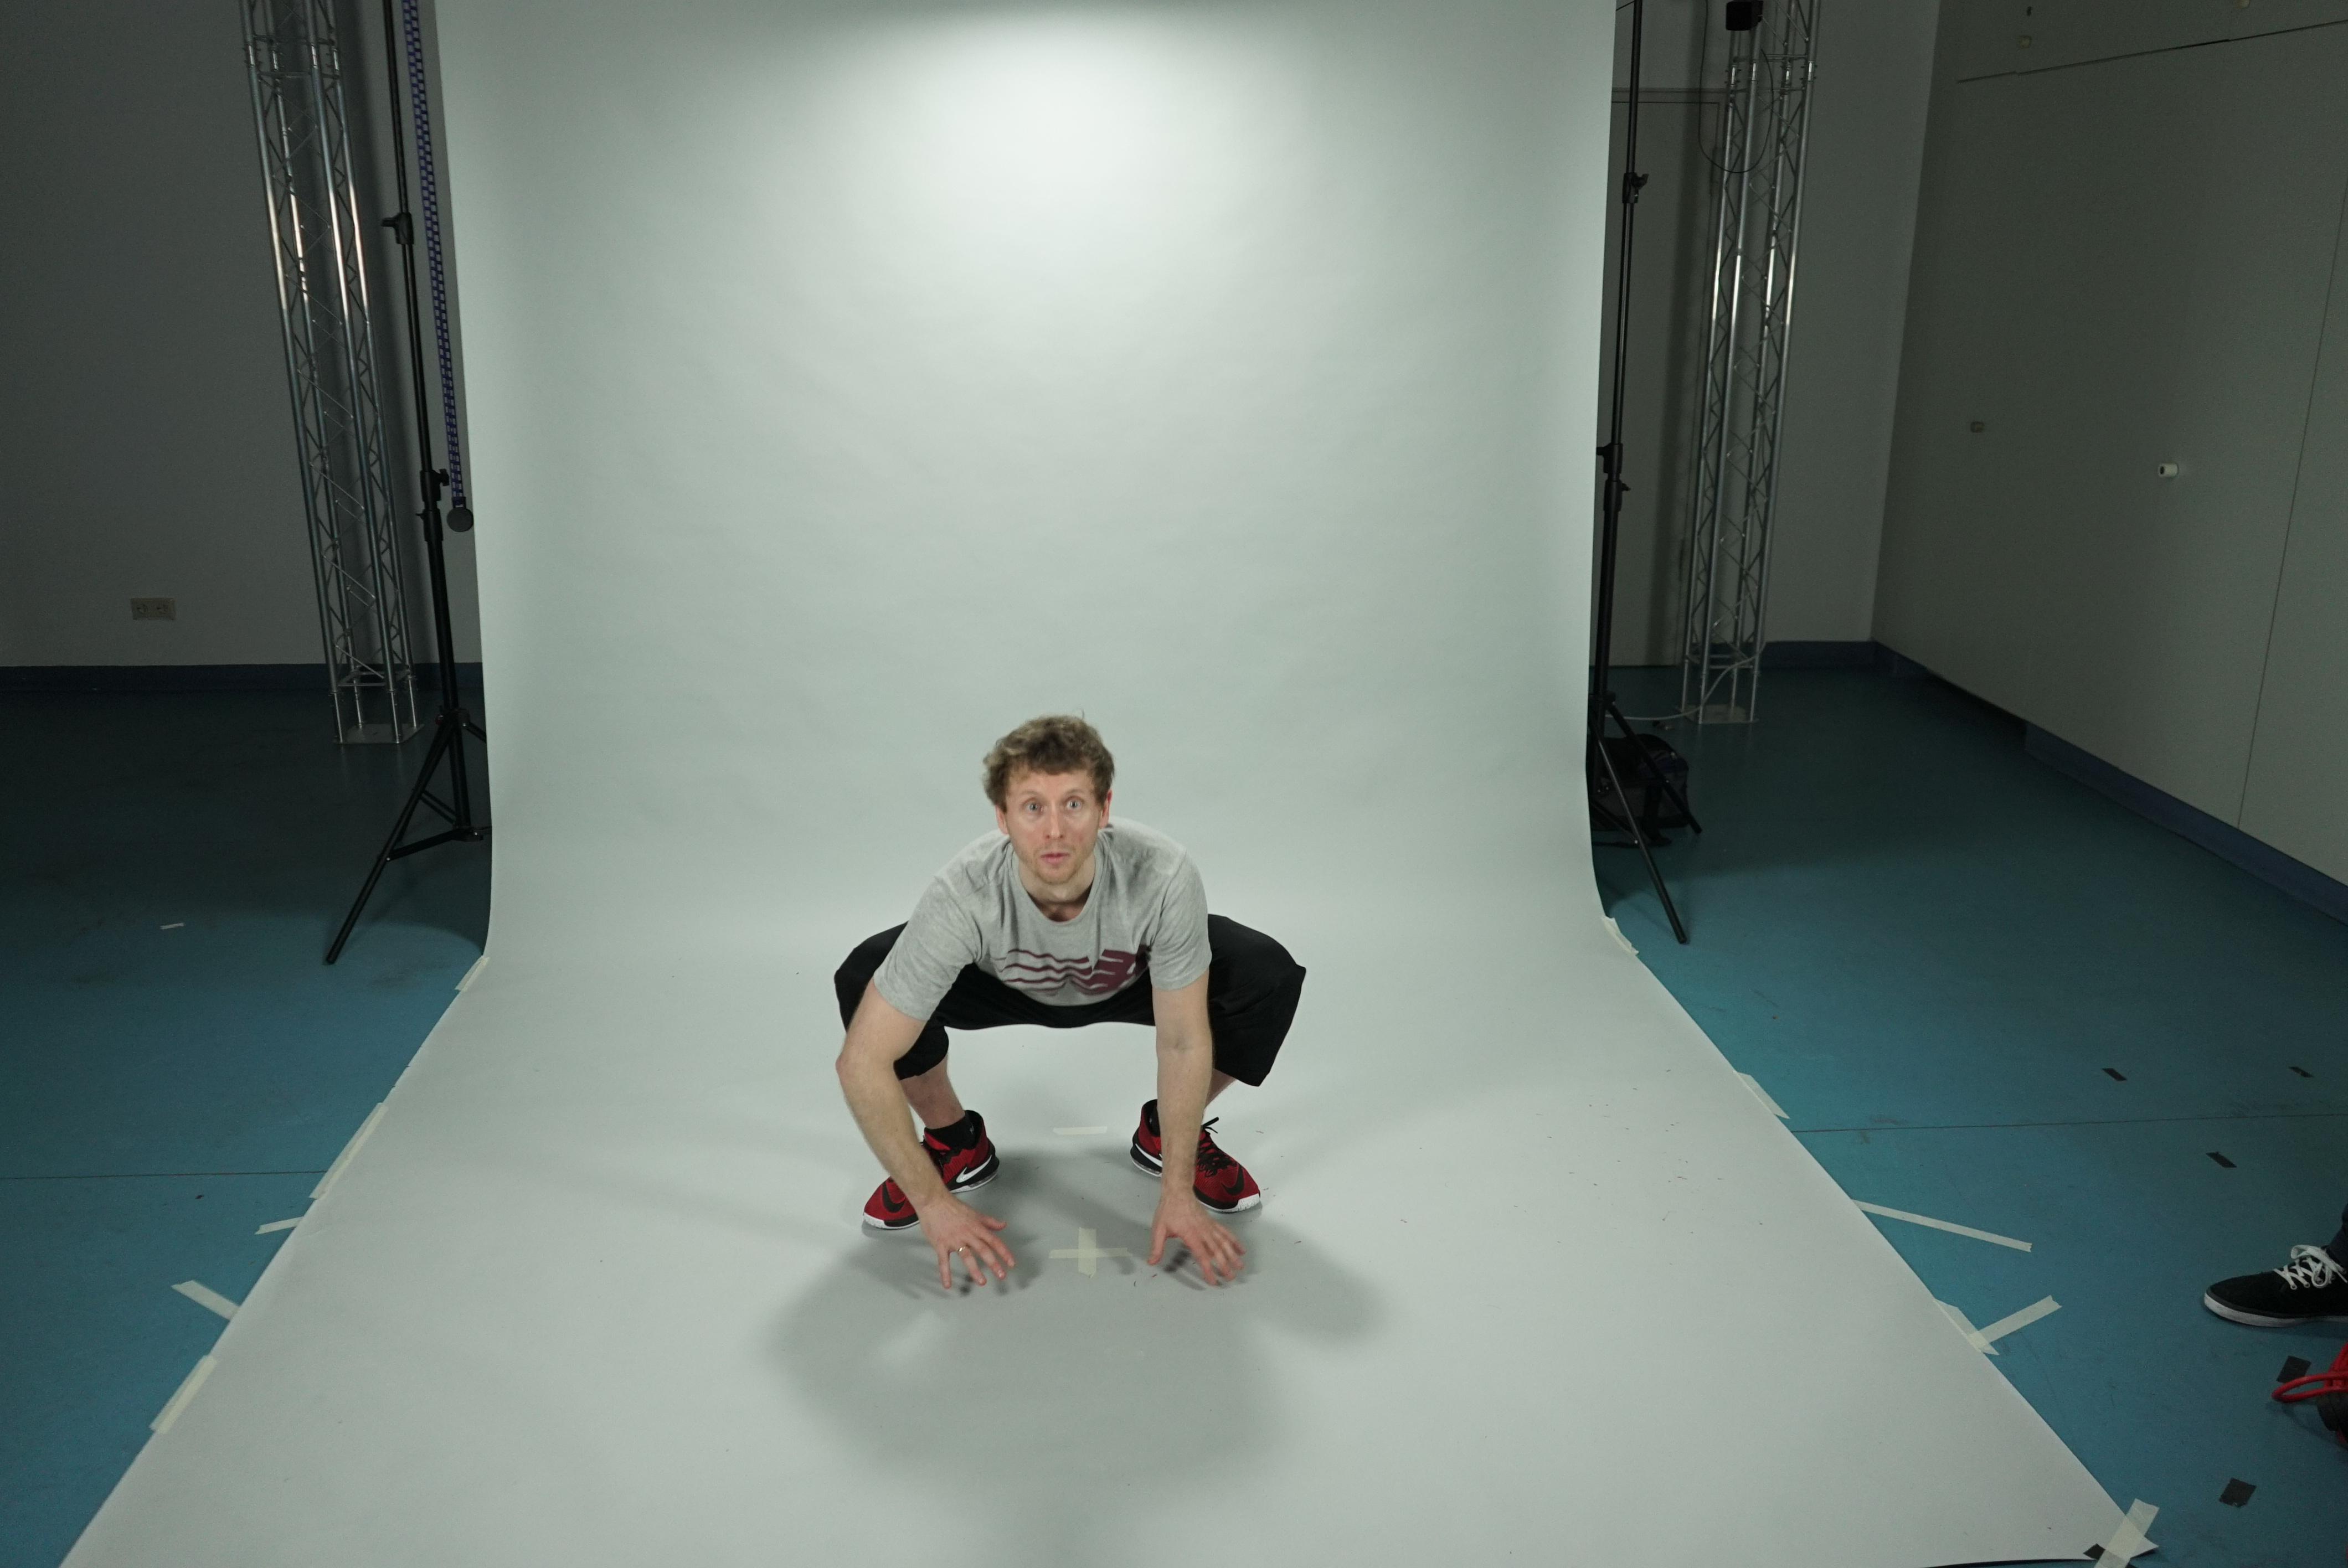
\includegraphics[width=0.85\textwidth]{ExpertSquat}
    \caption{Expert squat movement.}
    \label{fig:squatlong}
\end{figure}\\
Figure \ref{fig:bridge} is one of the filler segments used for the users to prepare for the next movement. However, in case the user does not use the bridge and comes in contact with the walls or lava obstacles, the user is looses a point.
\begin{figure}[h]
    \centering
    \includegraphics[width=0.85\textwidth]{Bridge}
    \caption{Bridge segment.}
    \label{fig:bridge}
\end{figure}\\
Figure \ref{fig:filler} depicts the filler (empty) segments that are placed at the beginning of the game and in between segments with obstacles in order to give players enough time to prepare for the subsequent movement.
\begin{figure}[h]
    \centering
    \includegraphics[width=\textwidth]{Filler1}
    \caption{Filler segments.}
    \label{fig:filler}
\end{figure}\\
Next, screenshots from game end will be presented and discussed in details.\pagebreak
\section{Game End Overview}
The player ends the game when she feels warmed up enough for the subsequent physical activity. When the game ends, the player is displayed the \textit{Individual score board} that is showed in Figure \ref{fig:individualend}.\\
\begin{figure}[h]
    \centering
    \includegraphics[width=\textwidth]{IndividualEndScene}
    \caption{Individual end scene.}
    \label{fig:individualend}
\end{figure}\\
Based on the player's username we display all the previous scores. The scores are displayed in descending order by the points achieved during each game run. The player is also presented with the duration each game lasted and the personal best score. By selecting the \textit{Back to main menu} button, the player can go back to the Home screen. 

\label{endgamelabel}
